% "Станет проще"

\documentclass[a4paper,12pt]{article} % тип документа

% report, book

%  Русский язык

\usepackage[T2A]{fontenc}			% кодировка
\usepackage[utf8]{inputenc}			% кодировка исходного текста
\usepackage{graphicx}
\usepackage[english,russian]{babel}	% локализация и переносы


%отступ
\usepackage[left=3cm,right=3cm,
    top=2cm,bottom=2cm,bindingoffset=0cm]{geometry}

% Математика
\usepackage{amsmath,amsfonts,amssymb,amsthm,mathtools} 
\usepackage{csvsimple}
\usepackage{multirow}

\usepackage{hyperref}
\usepackage{wasysym}
\usepackage{subcaption}
\usepackage{verbatim}
\usepackage{hyperref}
\usepackage{float}
\usepackage{enumerate}
\usepackage[dvipsnames]{xcolor}
\usepackage{rotating}
\usepackage{textcomp}

%Заговолок
%\graphicspath{ {images/} }


\begin{titlepage}
\author{Соловьянов Михаил }
\title{Задание 32. Влажность.}
\date{\today}
\end{titlepage}



\begin{document} % начало документа
\maketitle
%http://easyfizika.ru/zadachi/elektrostatika/

\section{ Задача на давление паров в газировке }

Студент купил в магазине теплую бутылку газировки. И решил открыть ее в момент времени $t_0$. Попробовав немного он подумал: <<Фу! Теплая!>>, после чего закрыв ее в момент времени  $t_1$ почти сразу же поставил в холодильник, где она медленно охлаждалась до температуры в 4\textdegree С. В момент времени $t_2$ студент достает бутылку из холодильника и опять открывает. Выпив половину он закрывает ее и оставляет на столе. После долгого времени, в момент времени $t_3$ он вновь открывает бутылку, однако оттуда вырывается еле слышимый <<Пшш>> После чего студент подумал <<Выдохлась>> и выбросил бытылку в момент времени $t_4$. Постройте графики:Температуру от времени $ T(t) $. Давления насыщенных паров воды в бутылке от времени $ P_np(t) $ . Влажности углекислого газа в бутылке от времени $ \varphi_{CO_2}(t) $. 


\begin{figure}[h]
\centering
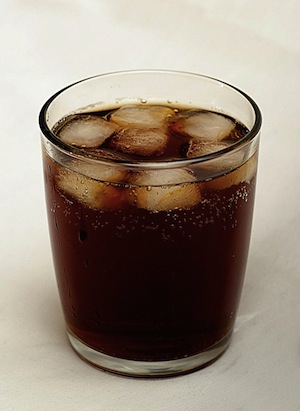
\includegraphics[width=0.5\textwidth]{cola.jpeg}
\end{figure}


\textit{Подсказка: графики строить один под другим.}



\end{document}